% !TeX root=../main.tex
\chapter{نظریه گراف}
%\thispagestyle{empty} 
\section{پیشگفتار} 
نظریه گراف نقش مهمی را در بسیاری از علوم دیگر بازی میکند، بسیاری از مفاهیم پیچیده از علوم فیزیک و شیمی گرفته تا علوم کامپیوتر توسط نظریه گراف توصیف میشود.
در این فصل علاوه بر مرور مختصر بر مفاهیم گراف، به الگوریتم هایی که در یافتن پاسخ خودکار مدار به ما یاری می رسانند پرداخته میشود.

\section{گراف}
گراف یک جفت مرتب
\footnote{
	گراف میتواند جهت دار یا بدون جهت باشد اگر گراف یاد شده بی جهت باشد استفاده از عبارت 
	«جفت» کافی است
	در غیر این صورت بایستی عبارت «جفت مرتب» را به کار برد. 
}
 به صورت
 $G = (V,E)$
 است به گونه ای که
  \lr{V}
 مجموعه ای از راس های گراف و
 $ E \subseteq \{(x,y)|(x,y) \in V^2 \}  $
 مجموعه یال های گراف است.
 با توجه به گستردگی نظریه گراف انواع زیادی از مفاهیم و الگوریتم ها درباره گراف موجود است
 ما در این فصل به توضیح آنچه که در پروژه استفاده شده بسنده خواهیم کرد.
\section{دور های ساده گراف}
اگر در یک گراف مجموعه ای از یال ها از یک راس مشخص شروع شده و با همان راس یاد شده خاتمه یابد
به آن مجموعه یک دور میگویم.
به دوری یک دور ساده
\LTRfootnote{simple cycle }
 گوییم هر آنگاه به جز راس نخستین و پایانی هیچ راس تکراری دیگری موجود نباشد یا به
 عبارت دیگر نتوان دور را به دور های کوچکتری شکست.
 
 به عنوان مثال در شکل
 \ref{fig:fig1} 
 دور
 \lr{ABDCA}
 یک دور ساده نیست چرا که میتواند به دو دور ساده
  \lr{ABCA}
  و
   \lr{BDCB}
   شکسته شود.
 
 \begin{figure}[ht]
 	\centerline{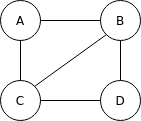
\includegraphics[width=5cm]{fig1}}
 	\caption{یک گراف بدون جهت شامل دو دور ساده}
 	\label{fig:fig1}
 \end{figure}
\subsection{پیدا کردن دور های ساده گراف}
پیدا کردن تمامی دور های ساده گراف از آن جهت برای ما اهمیت دارد که در مدل نهایی هر دور ساده
باعث یافتن یکی از
\LR{KVL}
موجود در مدار میشود.

برای یافتن مجموعه دور های ساده موجود در گراف ابتدا نیاز به یافتن درخت پوشای کمینه
\LTRfootnote{minimum spanning tree}
گراف یاد شده داریم، برای اینکار الگوریتم های زیادی از جمله الگوریتم کراسکال و
\LTRfootnote{kruskal}
الگوریتم پریم
\LTRfootnote{prim}
طراحی شده است، در پروژه حاضر از کتابخانه
\LR{networkx}
پایتون برای پیاده سازی استفاده شده است.

میتوان اثبات کرد که اگر یکی از یال های حذف شده را به درخت پوشای کمینه بیفزایم 
یک و تنها یک دور ساده ایجاد میشود که ما با الگوریتم
\LR{DFS}
\LTRfootnote{depth first search}
آن دور را می یابیم
، سپس با افزودن تمامی یال ها به صورت تک به تک تمامی دور های ساده یافت میشود.

به عنوان نمونه اگه گراف شکل
\ref{fig:fig1}
ورودی ما باشد درخت پوشای کمینه ما شکل
\ref{fig:fig2}
خواهد بود که دارای دو یال قطع شده
\lr{AB}
و
\lr{BD}
است.که با نقطه چین نمایش داده شده اند.
با اضافه کردن یال های قطع شده به صورت تک به تک دو گراف شکل
\ref{fig:fig3}
پدید می آیند که هر کدام دارای دارای یک دور ساده هستند سپس همانطور که یاد شد
با الگوریتم
\lr{DFS}
دور های مورد نظر را می یابیم.
\begin{figure}[ht]
	\centerline{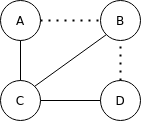
\includegraphics[width=5cm]{fig2}}
	\caption{درخت پوشای کمینه شکل
	\ref{fig:fig1} }
	\label{fig:fig2}
\end{figure}

\begin{figure}[ht]
	\centerline{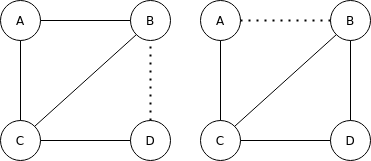
\includegraphics[width=9cm]{fig3}}
	\caption{دو گراف تک ساده دور شکل
		\ref{fig:fig1} }
	\label{fig:fig3}
\end{figure}


\subsection{شبه کد پیدا کردن دور های ساده گراف}
روند توضیح داده شده به صورت شبه کد، در الگوریتم 
 \eqref{simpcyc}
آمده است.
\begin{algorithm}[ht]
	\onehalfspacing
	\caption{الگوریتم پیدا کردن مجموعه دور های ساده گراف} 
	\label{simpcyc}
	\begin{algorithmic}[1]
		\REQUIRE
		 گراف
		\ENSURE
		 مجموعه دور های ساده گراف
		\STATE 
		درخت پوشای کمینه را پیدا کن.
		\STATE 
		یال های حذف شده از گراف برای تشکیل درخت را در یک استک ذخیره کن.
		\STATE
		یکی از یال های استک یاد شده را پاپ کن و به درخت پوشای کمینه اضافه کن و یک گراف تشکیل بده.
		\STATE
		گراف یاد شده دارای یک دور است آن دور را پیدا کن و به محموعه دور های ساده اضافه کن.
		\STATE
		اگر استک یاد شده خالی است به برنامه پایان بده در غیر این صورت به مرحله سوم برگرد.
	\end{algorithmic}
\end{algorithm}

\section{جمع بندی}